\documentclass[xcoler=dvipsnames, aspectratio=169]{beamer}

\usepackage{3191Style}
\newcommand{\C}{\mathbb{C}}
\newcommand{\F}{\mathbb{F}}
\newcommand{\abs}[1]{\left|#1\right|}
\renewcommand{\norm}[1]{\left\|#1\right\|}

% Date gives the title of the lecture
\date{Inner Products and Orthogonality}

\begin{document}
    \begin{frame}{Inner Product}
        Let $(V,\F)$ be a vector space where $V$ is the set our vectors come from and $\F$ is the 
        set our scalars come from (You can think of this as $\R$ or $\C$)\pause
        \begin{defn}
            \rText{Inner Product}: An \bText{inner product} is a function 
            $\ip{\cdot}{\cdot}:V\times V\rightarrow \F$ with the following properties for 
            all $\vec{u},\vec{v},\vec{w}\in V$, and $a,b\in\F$.
            \begin{enumerate}
                \pause\item $\ip{\vec{u}}{\vec{v}} = \overline{\ip{\vec{v}}{\vec{u}}}$\pause
                    \quad\text{Note: If $\F=\R$, then we omit the conjugate!}
                \pause\item $\ip{a\vec{u} + b\vec{v}}{\vec{w}} = a\ip{\vec{u}}{\vec{w}} + 
                    b\ip{\vec{v}}{\vec{w}}$
                \pause\item $\ip{\vec{v}}{\vec{v}}\geq 0$
                \pause\item $\ip{\vec{v}}{\vec{v}} = 0$ if and only if $\vec{v}=\vec{0}$.
            \end{enumerate}
        \end{defn}
    \end{frame}
    \begin{frame}{Inner Product Example: $\C^n$ (standard) Part 1}
        Let $V=\C^n$ and $\F=\C$. Then the following function is an inner product
        \[
            \ip{\vec{x}}{\vec{y}} = \overline{\vec{y}}^\top\vec{x} = \sum_{k=1}^n x_k\overline{y_k}
        \]\pause
        {\let\thefootnote\relax\footnotetext{
            {Note: we sometimes abbreviate $\overline{\vec{y}}^\top$ as $\vec{y}^*$}}}

        Note that if we are in the real numbers, then we omit the conjugate of $\vec{y}$.
    \end{frame}
    \begin{frame}{Inner Product Example: $\C^n$ (standard) Part 2}
        Property 1: $\ip{\vec{x}}{\vec{y}} = \overline{\ip{\vec{y}}{\vec{x}}}$\pause
        \[
            \ip{\vec{x}}{\vec{y}}\pause = \sum_{k=1}^n x_k\overline{y_k}
            \pause = \sum_{k=1}^n \overline{y_k}x_k
            \pause = \sum_{k=1}^n \overline{\overline{\overline{y_k}x_k}}
            \pause = \overline{\sum_{k=1}^ny_k\overline{x_k}}\pause = \overline{\ip{\vec{y}}{\vec{x}}}
        \]\pause
        Property 2: $\ip{a\vec{x} + b\vec{y}}{\vec{z}} = a\ip{\vec{x}}{\vec{z}} + b\ip{\vec{y}}{\vec{z}}$
        \pause
        \[
            \ip{a\vec{x} + b\vec{y}}{\vec{z}}\pause = \sum_{k=1}^n(ax_k + by_k)\overline{z_k}
            \pause = \sum_{k=1}^n ax_k\overline{z_k} + by_k\overline{z_k}
            \pause = \sum_{k=1}^n ax_k\overline{z_k} + \sum_{k=1}^n by_k\overline{z_k}
            \pause = a\ip{\vec{x}}{\vec{z}} + b\ip{\vec{y}}{\vec{z}}
        \]
    \end{frame}
    \begin{frame}{Inner Product Example: $\C^n$ (standard) Part 3}
        Property 3,4: $\ip{\vec{x}}{\vec{x}}\geq 0$ and $\ip{\vec{x}}{\vec{x}} = 0$ if and only if
        $\vec{x} = \vec{0}$
        \[
            \ip{\vec{x}}{\vec{x}}\pause = \sum_{k=1}^n x_k\overline{x_k}
            \pause = \sum_{k=1}^n \abs{x_k}^2\pause \geq 0
        \]\pause
        In addition, the only time $\sum_{k=1}^n \abs{x_k}^2=0$ is when all components are 0 or 
        if $\vec{x}=\vec{0}$
    \end{frame}
    \begin{frame}{Dot Product}
        \begin{defn}
            \rText{Dot Product}: The \bText{dot product} of two vectors in $\R^n$ is a function given by
            \[
                \ip{\vec{x}}{\vec{y}} = \vec{y}^\top\vec{x}
            \]
        \end{defn}\pause
        \begin{theorem}
            The \bText{dot product} is an inner product.
        \end{theorem}\pause
        \begin{proof}
            The 2 previous slides prove this.
        \end{proof}\pause
        Note: For this course, we will only consider this inner product unless stated otherwise
    \end{frame}
    \begin{frame}{Norms}
        Let $(V,\F)$ be a vector space where $V$ is the set our vectors come from and $\F$ is the 
        set our scalars come from (You can think of this as $\R$ or $\C$)\pause
        \begin{defn}
            \rText{Norm}: A \bText{norm} is a function given by $\norm{\cdot}:V\rightarrow\R$
            with the following properties for all $\vec{x},\vec{y}\in V$ and $c\in\F$
            \begin{enumerate}
                \pause\item $\norm{\vec{x} + \vec{y}}\leq \norm{\vec{x}} + \norm{\vec{y}}$
                \pause\item $\norm{c\vec{x}} = \abs{c}\norm{\vec{x}}$
                \pause\item $\norm{\vec{x}} = 0$ if and only if $\vec{x} = \vec{0}$
            \end{enumerate}
        \end{defn}
    \end{frame}
    \begin{frame}{Induced Norms}
        \begin{theorem}
            Let $(V,\F)$ be a vector space with some inner product $\ip{\cdot}{\cdot}$. Then the
            \bText{induced norm} of this space is
            \[
                \norm{\vec{x}} = \sqrt{\ip{\vec{x}}{\vec{x}}}
            \]
        \end{theorem}\pause
        \begin{proof}
            We can prove all 3 properties from the previous slide as consequences of us using the
            inner product.
        \end{proof}
    \end{frame}
    \begin{frame}{Example of a Norm}
        If $V=\R^n$ and $\F=\R$, then the induced norm is often called the ``Euclidean Norm'' and
        denoted as follows\pause
        \[
            \norm{\vec{x}}_2 = \sqrt{\vec{x}^\top\vec{x}}\pause = \sqrt{\sum_{k=1}^nx_k^2}
        \]\pause

        For this course, we will consider only this norm unless stated otherwise.
    \end{frame}
    \begin{frame}{Unit Vector}
        \begin{defn}
            \rText{Unit Vector}: We say a vector is a \bText{unit vector} if it has norm 1. In
            other words, $\vec{x}$ is a unit vector if and only if
            \[
                \norm{\vec{x}} = 1
            \]
        \end{defn}
        \pause
        If we have any vector, $\vec{x}\neq\vec{0}$, then we can find a vector pointing in the same
        direction, but is also of \emph{unit length} by doing:
        \[
            \vec{y} = \frac{\vec{x}}{\norm{\vec{x}}}
        \]
    \end{frame}
    \begin{frame}{Distance}
        For us, we can think of distance between vectors as ``how large is the difference between
        two vectors'', or in other words, we say
        \[
            d(\vec{x},\vec{y}) = \norm{\vec{y}-\vec{x}}
        \]

        Note: this idea is closely related to ``Metric Spaces''\footnote{\url{https://en.wikipedia.org/wiki/Metric\_space\#Definition}}, which you will see in an analysis course.
    \end{frame}
    \begin{frame}{Angle Between Vectors}
        \small
        \begin{center}
            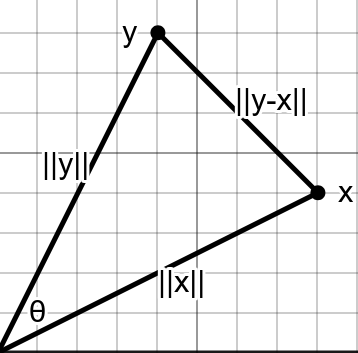
\includegraphics[width=.15\textwidth]{images/lawOfCosines2.png}
        \end{center}
        \pause
        \begin{columns}
            \column{.5\textwidth}
            Using the law of cosines\footnote{\url{https://en.wikipedia.org/wiki/Law\_of\_cosines}},
            we have that 
            \[
                \norm{\vec{y}-\vec{x}}^2 = \norm{\vec{x}}^2 + \norm{\vec{y}}^2 
                -2\norm{\vec{x}}\norm{\vec{y}}\cos(\theta)
            \]\pause
            \vspace{-10pt}
            \[
                (\vec{y}-\vec{x})^\top(\vec{y} - \vec{x}) = \vec{x}^\top\vec{x} + \vec{y}^\top\vec{y}
                - 2\norm{\vec{x}}\norm{\vec{y}}\cos(\theta)
            \]\pause
            \column{.5\textwidth}
            Which (assuming that $\vec{x},\vec{y}\neq\vec{0}$) can be solved for $\theta$ to get
            \[
                \theta = \cos^{-1}\left(\frac{\vec{x}^\top\vec{y}}{\norm{\vec{x}}\norm{\vec{y}}}\right)
            \]\pause
            In higher dimensions and other vector spaces, this is how we define the angle between vectors
        \end{columns}
    \end{frame}
    \begin{frame}{Orthogonality}
        Let $(V,\F)$ be a vector space where $V$ denotes the set our vectors come from, $\F$ is the
        set our scalars come from, and we have some inner product $\ip{\cdot}{\cdot}$.
        \begin{defn}
            \rText{Orthogonal Vectors}: We say that 2 vectors, 
            ($\vec{x},\vec{y}\in V$) are \bText{orthogonal} (or \bText{perpendicular}) if
            \[
                \ip{\vec{x}}{\vec{y}} = 0
            \]\pause
        \end{defn}
        Note that assuming we have non-zero vectors, the angle between $\vec{x},\vec{y}$ 
        would be $90^\circ$!\pause
        \begin{tcolorbox}
            Since orthogonality is closely tied to our inner product, we will use our standard one
            for this course.
        \end{tcolorbox}
    \end{frame}
    \begin{frame}{Special Case for Orthogonality}
        \begin{theorem}
            If $V=\R^n$ (or equivalently $\C^n$) with the usual inner product, then $\vec{0}$ is 
            orthogonal to every vector.
        \end{theorem}
        \vspace{50pt}
        \begin{proof}
            Let $\vec{x}\in\R^n$ and $\ip{\cdot}{\cdot}$ denote the standard inner product, then
            we have that
            \[
                \ip{\vec{0}}{\vec{x}}\pause = \sum_{k=1}^n 0\cdot x_k = 0
            \]
        \end{proof}
    \end{frame}
\end{document}
